\section*{K3/4. feladat: Rugót tehermentesítő vízsugár} 
\addcontentsline{toc}{section}{K3/4. feladat}

%feladatleírás
Mekkora sebességgel kell kilépni az ábrán látható csőből a vízsugárnak, hogy a rugót éppen tehermentesítse?
Az ábra a víz indulása \textbf{előtti} állapotot ábrázolja.
Készítsen a ható erőkről vektorábrát! 
Veszteségmentes áramlást tételezünk fel, az $m$ tömegű tárgy mérete elhanyagolható.

%megadott_adatok
\begin{equation*}
	H = \SI{0,2}{\meter},
	\quad
	d = \SI{50}{\milli\meter}, 
	\quad
	q_v = \SI{10e3}{\kilogram\per\meter\cubed},
	\quad
	m = \SI{1}{\kilogram},
	\quad
	c_r = \SI{5}{\milli\meter\per\newton},
	\quad
	g = \SI{9,81}{\meter\per\second\squared}
	\end{equation*}

\begin{figure}[h]
	\centering
	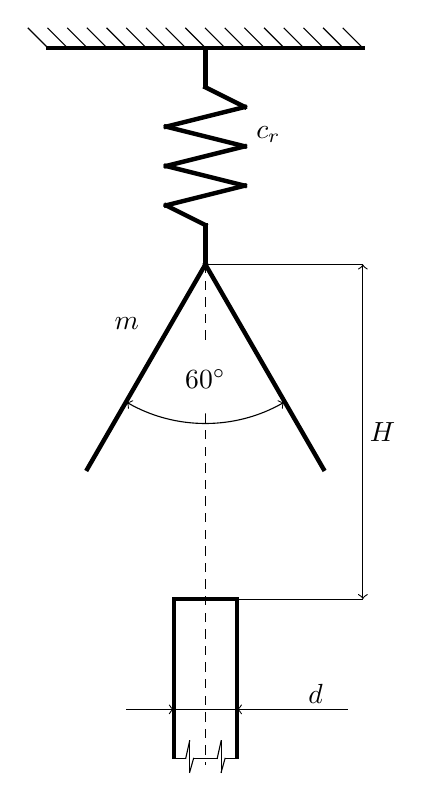
\begin{tikzpicture}[every path/.style={line cap=rect}][scale=5]
%talaj rész
\draw [ultra thick](0,-1) -- (4,-1);
%szagatott vonalazás
\draw (0,-1) -- (-0.25,-0.75);
\draw (0.25,-1) -- (0,-0.75);
\draw (0.5,-1) -- (0.25,-0.75);
\draw (0.75,-1) -- (0.5,-0.75);
\draw (1,-1) -- (0.75,-0.75);
\draw (1.25,-1) -- (1,-0.75);
\draw (1.5,-1) -- (1.25,-0.75);
\draw (1.75,-1) -- (1.5,-0.75);
\draw (2,-1) -- (1.75,-0.75);
\draw (2.25,-1) -- (2,-0.75);
\draw (2.5,-1) -- (2.25,-0.75);
\draw (2.75,-1) -- (2.5,-0.75);
\draw (3,-1) -- (2.75,-0.75);
\draw (3.25,-1) -- (3,-0.75);
\draw (3.5,-1) -- (3.25,-0.75);
\draw (3.75,-1) -- (3.5,-0.75);
\draw (4,-1) -- (3.75,-0.75);
%rugó
\draw [ultra thick](2,-1) -- (2,-1.5);
\draw [ultra thick](2,-1.5) -- (2.5,-1.75);
\draw [ultra thick](2.5,-1.75) -- (1.5,-2);
\draw [ultra thick](1.5,-2) -- (2.5,-2.25); 
\node at (2.8,-2.1){$c_r$};
\draw [ultra thick](2.5,-2.25) -- (1.5,-2.5);
\draw [ultra thick](1.5,-2.5) -- (2.5,-2.75);
\draw [ultra thick](2.5,-2.75) -- (1.5,-3);
\draw [ultra thick](1.5,-3) -- (2,-3.25);
\draw [ultra thick](2,-3.25) -- (2,-3.75);
%rugó alatti tányér
\draw [ultra thick] (2,-3.75) -- ++ (60:-3cm);
\draw [ultra thick] (2,-3.75) -- ++ (120:-3cm);
\draw [<->] (1,-5.5) arc (240:300:2 cm);
\node at (1,-4.5){$m$};
%cső
\draw [dashed] (2,-3.75) -- (2,-10.1);
\node at (2,-5.2)[circle,fill=white]{$60^\circ$};
\draw [ultra thick] (2.40,-10) -- (2.40,-8);
\draw [ultra thick] (1.60,-10) -- (1.60,-8);
\draw [ultra thick] (2.40,-8) -- (1.60,-8);
\draw (2.40,-10.023) -- (2.25,-10.023);
\draw (2.25,-10.023) --(2.2,-10.2);
\draw (2.2,-10.2) -- (2.2,-9.8);
\draw (2.2,-9.8) -- (2.15,-10.023);
\draw (2.15,-10.023) -- (1.85,-10.023);
\draw (1.85,-10.023) -- (1.80,-10.2);
\draw (1.80,-10.2) -- (1.80,-9.8);
\draw (1.80,-9.8) -- (1.75,-10.023);
\draw (1.75,-10.023) -- (1.60,-10.023);
\draw (1.3,-9.4) -- (2.7,-9.4);
\draw [->](1,-9.4) -- (1.60,-9.4);
\draw [->](3.8,-9.4) -- (2.40,-9.4);
\node at (3.40,-9.2){$\diameter d$};
%magasság
\draw (2.40,-8) -- (4,-8);
\draw [<->] (4,-8) -- (4,-3.75);
\node at (4.25,-5.875){$H$};
\draw (2,-3.75) -- (4,-3.75);
	\end{tikzpicture}
	\caption{A vízsugár elindulása előtti állapot vázlata.}
	\label{figure:K34A}
\end{figure}
\subsubsection*{1. Rugóerő vizsgálata}
Az $m$ tömegű teher kényszeríti a rugót a megnyúlásra, ennek hatására ébred az ellenkező irányba $\vec{F_r}$ rugóerő.
\begin{equation}
	m  \vec{g} = \vec{F_r} = \frac{\Delta h}{\vec{c_r}}
\end{equation}
\begin{equation}
\Delta h = \vec{c_r}  m  \vec{g} = \SI{49}{\milli\meter}
\end{equation}

\subsubsection*{2. Imulzuserők vizsgálata}
\begin{equation}
	\vec{J_{BE}} + \vec{J_{KI1}} + \vec{J_{KI2}} = \vec{F_r} = m \vec{g}
\end{equation}
\begin{equation}
\vec{J_{BE}} = \dot{m} v_2 = \varrho_v \frac{d^2 \pi}{4} v_1 v_2
\end{equation}
\begin{equation}
\vec{J_{KI1}} = \vec{J_{KI2}} = \frac{1}{2} \dot{m} v_2 = \frac{1}{2} \varrho_v \frac{d^2 \pi}{4} v_1 v_2
\end{equation}
\begin{equation}
\vec{J_{BE}} + \vec{J_{KI1}} \cos\alpha + \vec{J_{KI2}} \cos\alpha = mg  
\end{equation}
\begin{equation}
\alpha = \frac{1}{2} \cdot 60^\circ
\end{equation}
\begin{equation}
\varrho_v \frac{d^2 \pi}{4} v_1 v_2 (1+\cos\alpha) = m g 
\end{equation}

\begin{figure}[h]
	\centering
	\begin{subfigure}[b]{0.33\textwidth}
	\centering
	\begin{tikzpicture}
	%vízsugár kitöltése
	\draw [cyan, fill=cyan,ultra thick] (1.60,-4.75) -- (1.60,-7.95) -- (2.40,-7.95) -- (2.40,-4.75) -- ++ (120:-1.23) -- (3.48,-5.65) -- ++ (120:3) -- ++ (60:-2.9cm) -- ++ (337:0.52) -- (1.60,-4.75);
	%talaj rész
	\draw [ultra thick](0,-1) -- (4,-1);
	%szagatott vonalazás
	\draw (0,-1) -- (-0.25,-0.75);
	\draw (0.25,-1) -- (0,-0.75);
	\draw (0.5,-1) -- (0.25,-0.75);
	\draw (0.75,-1) -- (0.5,-0.75);
	\draw (1,-1) -- (0.75,-0.75);
	\draw (1.25,-1) -- (1,-0.75);
	\draw (1.5,-1) -- (1.25,-0.75);
	\draw (1.75,-1) -- (1.5,-0.75);
	\draw (2,-1) -- (1.75,-0.75);
	\draw (2.25,-1) -- (2,-0.75);
	\draw (2.5,-1) -- (2.25,-0.75);
	\draw (2.75,-1) -- (2.5,-0.75);
	\draw (3,-1) -- (2.75,-0.75);
	\draw (3.25,-1) -- (3,-0.75);
	\draw (3.5,-1) -- (3.25,-0.75);
	\draw (3.75,-1) -- (3.5,-0.75);
	\draw (4,-1) -- (3.75,-0.75);
	%rugó
	\draw [ultra thick](2,-1) -- (2,-1.5);
	\draw [ultra thick](2,-1.5) -- (2.5,-1.625);
	\draw [ultra thick](2.5,-1.625) -- (1.5,-1.75);
	\draw [ultra thick](1.5,-1.75) -- (2.5,-1.875); 
	\node at (2.8,-2){$c_r$};
	\draw [ultra thick](2.5,-1.875) -- (1.5,-2);
	\draw [ultra thick](1.5,-2) -- (2.5,-2.125);
	\draw [ultra thick](2.5,-2.125) -- (1.5,-2.25);
	\draw [ultra thick](1.5,-2.25) -- (2,-2.5);
	\draw [ultra thick](2,-2.5) -- (2,-3);
	
	%rugó alatti tányér
	\draw [ultra thick] (2,-3) -- ++ (60:-3cm);
	\draw [ultra thick] (2,-3) -- ++ (120:-3cm);
	\node at (1,-2){$\vec{0}N$};
	
	%cső
	\draw [ultra thick] (2.40,-10.023) -- (2.40,-8);
	\draw [ultra thick] (1.60,-10.023) -- (1.60,-8);
	\draw [ultra thick] (2.40,-8) -- (1.60,-8);
	\draw (2.40,-10.023) -- (2.25,-10.023);
	\draw (2.25,-10.023) --(2.2,-10.2);
	\draw (2.2,-10.2) -- (2.2,-9.8);
	\draw (2.2,-9.8) -- (2.15,-10.023);
	\draw (2.15,-10.023) -- (1.85,-10.023);
	\draw (1.85,-10.023) -- (1.80,-10.2);
	\draw (1.80,-10.2) -- (1.80,-9.8);
	\draw (1.80,-9.8) -- (1.75,-10.023);
	\draw (1.75,-10.023) -- (1.60,-10.023);
	
	%vízsugár
	\draw [blue] [ultra thick] (2.40,-7.95) -- (1.60,-7.95);
	\draw [blue] [ultra thick] (2.40,-7.99) -- (2.40,-4.75);
	\draw [blue] [ultra thick] (1.60,-7.99) -- (1.60,-4.75);
	\draw [blue] [ultra thick] (1.60,-4.75) -- ++ (60:-1.25);
	\draw [blue] [ultra thick] (2.40,-4.75) -- ++ (120:-1.25);
	\draw [blue , fill=cyan] [ultra thick] (0.72,-5.75) ellipse (7.5pt and 6pt);
	\draw [blue , fill=cyan] [ultra thick] (3.28,-5.75) ellipse (7.5pt and 6pt);
	\draw [blue , fill=cyan] [ultra thick] [dashed] (2,-6.5) ellipse (11pt and 4pt);
	
	%áramlás_iránya
	\draw (2,-7.95) -- (3.28,-9 )node[anchor=north west ,circle,draw]{1};
	\draw [red] [fill] (2,-7.95) circle [radius=0.05];
	\draw (2,-3.1) -- (3.28,-2.5)node[anchor=south west ,circle,draw]{2};
	\draw [red] [fill] (2,-3.1)circle [radius=0.05];
	\draw [mid arrow=red, red, ultra thick] (2,-8) -- (2,-3.1); 
	
	\end{tikzpicture}
	\caption{A vízsugár elindulása után keletkező állapot.}	
	\end{subfigure}
	\begin{subfigure}[b]{0.31\textwidth}
	\centering
	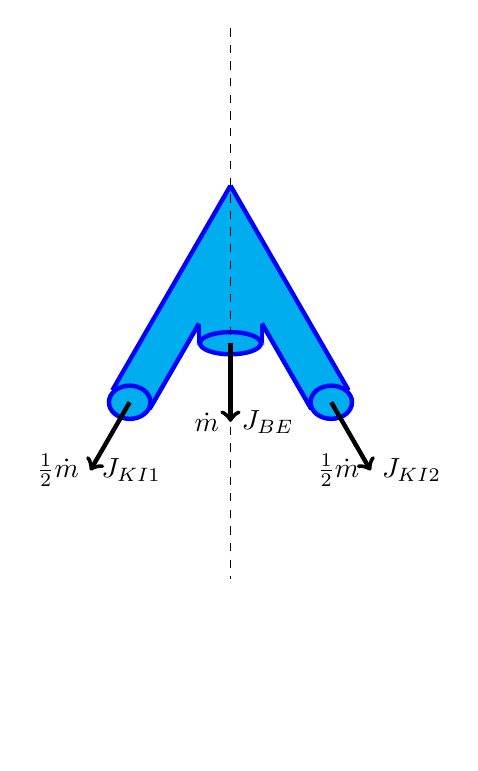
\begin{tikzpicture}
	%vízsugár kitöltése
	\draw [cyan, fill=cyan,ultra thick] (1.60,-4.75) -- (1.60,-5) -- (2.40,-5) -- (2.40,-4.75) -- ++ (120:-1.23) -- (3.48,-5.65) -- ++ (120:3) -- ++ (60:-2.9cm) -- ++ (337:0.52) -- (1.60,-4.75);
	%vízsugár
	\draw [blue] [ultra thick] (2,-3) -- ++ (60:-3cm);
	\draw [blue] [ultra thick] (2,-3) -- ++ (120:-3cm);
	\draw [blue] [ultra thick] (2.40,-5) -- (1.60,-5);
	\draw [blue] [ultra thick] (2.40,-5) -- (2.40,-4.75);
	\draw [blue] [ultra thick] (1.60,-5) -- (1.60,-4.75);
	\draw [blue] [ultra thick] (1.60,-4.75) -- ++ (60:-1.25);
	\draw [blue] [ultra thick] (2.40,-4.75) -- ++ (120:-1.25);
	\draw [blue , fill=cyan] [ultra thick] (0.72,-5.75) ellipse (7.5pt and 6pt);
	\draw [blue , fill=cyan] [ultra thick] (3.28,-5.75) ellipse (7.5pt and 6pt);
	\draw [blue , fill=cyan] [ultra thick] (2,-5) ellipse (11pt and 4pt);
	\draw [dashed] (2,-1) -- (2,-8);
	
	%impulzus erők
	\draw [ultra thick][->](2,-5) -- (2,-6) node[anchor=east]{$\dot{m}$} node[anchor=west]{$J_{BE}$};
	\draw [ultra thick][->](0.72,-5.75) -- ++ (60:-1) node[anchor=east]{$\frac{1}{2}\dot{m}$} node[anchor=west]{$J_{KI1}$} ;
	\draw [ultra thick][->](3.28,-5.75) -- ++ (120:-1) node[anchor=east]{$\frac{1}{2}\dot{m}$} node[anchor=west]{$J_{KI2}$} ;
	\draw [white] [fill] (2,-10.023)circle [radius=0.05];
	\end{tikzpicture}
	\caption{A vízsugárra ható impulzus erők és irányuk.}			
	\end{subfigure}
	\begin{subfigure}[b]{0.3\textwidth}
	\centering
	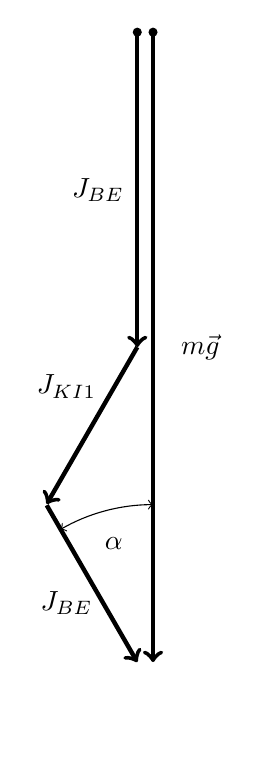
\begin{tikzpicture}
	%vektorábra
	\draw [fill] (2,0)circle [radius=0.05];
	\draw [fill] (1.8,0)circle [radius=0.05];
	\draw [ultra thick][->] (2,0) -- (2,-8);
	\node at (2.6,-4) {$m\vec{g}$};
	\draw [ultra thick][->] (1.8,0) -- (1.8,-4);
	\node at (1.3,-2) {$J_{BE}$};
	\draw [ultra thick][->] (1.8,-2*2) -- ++ (240: 1.15*2);
	\draw [ultra thick][<-] (1.8,-4*2) -- ++ (120: 1.15*2);
	\node at (0.9,-4.5) {$J_{KI1}$};
	\node at (0.9,-7.25) {$J_{BE}$};
	\draw [<->] (2,-6) arc (90:120:2.35 cm); 
	\node at (1.5,-6.5)[circle,fill=white]{$\alpha$};
	\draw [white] [fill] (2,-9)circle [radius=0.05];
	\end{tikzpicture}
	\caption{A ható erők vektorábrája.}		
	\end{subfigure}
	\label{figure:K34A}
\end{figure}
\subsubsection*{3. Veszteségmentes Bernulli egyenlet}
\begin{equation}
	\frac{v_{1}^2}{2} + \frac{p_1}{\varrho_v} + g z_1 = \frac{v_{2}^2}{2} + \frac{p_2}{\varrho_v} + g z_2
\end{equation}
\begin{equation*}
	p_1 = p_2 = p_0, 
	\quad
	z_1 = \SI{0}{\meter},
	\quad
	z_2 = H + \Delta h
\end{equation*}
\begin{equation}
	v_{1}^2 = v_{2}^2 + 2g(H + \Delta h)
	 v_{2} = \frac{mg}{\varrho_v \frac{d^2\pi}{4}(1+\cos\alpha)v_1} = \frac{\SI{2,67}{\meter\squared\per\second\squared}}{v_1}
\end{equation}
\begin{equation}
	v_{1}^2 = \frac{\SI{7,168}{\frac{\meter^4}{\second^4}}}{v_{1}^2} + \SI{4,88}{\meter\squared\per\second\square}
\end{equation}
\begin{equation}
	v_1^4 - \SI{4,88}{\meter\squared\per\second\square} v_{1}^2 - \SI{7,168}{\frac{\meter^4}{\second^4}} = \SI{0}{}
\end{equation}
\begin{equation}
	v_1 = x
\end{equation}
\begin{equation}
	x^4 - \SI{4,88}{x^2} - \SI{7,169}{} = \SI{0}{}
\end{equation}
\begin{equation}
	\underbrace{
		\left(x_1 = \SI{-1,181}{\meter\squared\per\second\square}\right)
	}_{\substack{\text{a másodfokú egyenletnek megoldása,} \\ \text{de a fizikai problémának nem}}}
	,
	\quad
	x_2 = \SI{6,067}{\meter\squared\per\second\square}
	\quad
	\Rightarrow
	\quad
	v_1 = \sqrt{x_2} = \SI{2,463}{\meter\per\second}
\end{equation}
\pagebreak